\documentclass[border=6pt]{standalone}
\usepackage{tikz}
\usetikzlibrary{arrows.meta,positioning,shapes.geometric,shapes.multipart,calc,fit,backgrounds,decorations.pathreplacing,decorations.markings,automata,chains,matrix,patterns}
\usepackage{circuitikz}
\usepackage{amsmath}
\usepackage{amssymb}
\begin{document}
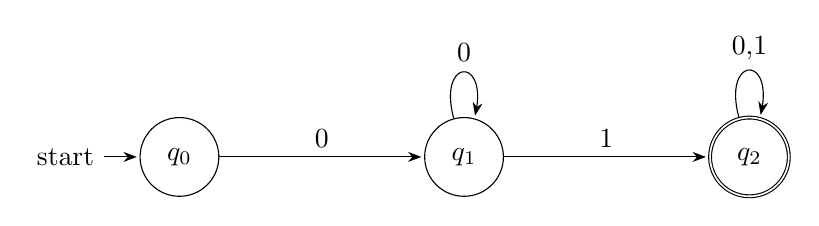
\begin{tikzpicture}[
  ->, >=Stealth, shorten >=1pt, auto, node distance=2.6cm,
  state/.style={circle, draw, minimum size=1cm}
]
  \node[state, initial] (q0) {$q_0$};
  \node[state, right=of q0] (q1) {$q_1$};
  \node[state, accepting, right=of q1] (q2) {$q_2$};

  \path (q0) edge node {0} (q1)
        (q1) edge node {1} (q2)
        (q1) edge [loop above] node {0} (q1)
        (q2) edge [loop above] node {0,1} (q2);
\end{tikzpicture}
\end{document}
